\documentclass[conference]{IEEEtran}
\usepackage{times}

% numbers option provides compact numerical references in the text.
\usepackage[numbers]{natbib}
\usepackage{multicol}
\usepackage[bookmarks=true]{hyperref}
% --- additions below do not change the template's fonts, page size or spacing ---
\usepackage{graphicx}
\usepackage{booktabs}
\usepackage{amsmath}
\usepackage{xcolor}

\pdfinfo{
   /Author (Anonymous)
   /Title  (When Does Soft Tissue Matter for Robot Learning in Ultrasound?)
   /Subject (Robotic ultrasound; soft-tissue simulation; robot learning)
   /Keywords (robotic ultrasound; deformable simulation; finite element; reinforcement learning; pre-registration)
}

\newcommand{\RM}{\textsc{r}}   % rigid mode
\newcommand{\KM}{\textsc{k}}   % kinematic mode
\newcommand{\DM}{\textsc{d}}   % deformable mode

\begin{document}

\title{When Does Soft Tissue Matter for Robot Learning\\ in Ultrasound? A Pre-Registered Study on\\
Patient-Specific Deformable Anatomy}

\author{Author Names Omitted for Anonymous Review. Paper-ID [add your ID here]}

\maketitle

\begin{abstract}
Robot-learning simulators for ultrasound treat the patient as rigid, although a probe can only image by pressing on
soft tissue. Whether this simplification matters has not been measured. We pose it as a falsifiable question and
answer it with a simulator in which each of 13 CT patients has a GPU-batched finite-element model of the soft tissue,
a force-controlled probe, and B-mode images rendered from the deformed anatomy. The key methodological device is a
\emph{kinematic} control mode that presses the probe into undeformed tissue; it splits any rigid-versus-deformable
difference into a part due to probe indentation, which a rigid simulator can reproduce, and a part due to deformation,
which it cannot. All hypotheses, thresholds and analysis scripts are fixed before each run. Preliminary results give
one positive and one negative answer. (i)~A soft-tissue \emph{measurement} depends on deformation: paraspinal muscle
thickness read from the image falls by 0.25--0.30\,mm/N on held-out patients, tracking the true compression, while
the rigid control stays within $\pm$0.04\,mm/N. (ii)~\emph{Policy behaviour} in navigation does not: policies trained
with and without deformation differ by $-0.8$ success points, and the residual gap to rigid training is explained
by indentation. We propose to test whether deformation changes behaviour once the policy controls the contact force,
and to scale the measurement result to many patients.
\end{abstract}

\IEEEpeerreviewmaketitle

% =====================================================================================================
\section{Introduction}

An ultrasound probe must press on the body to form an image, and pressing deforms the tissue under it. Robotic
ultrasound systems therefore regulate contact force~\cite{jiang2023review}, and image-processing work corrects the
resulting deformation in reconstructed volumes~\cite{burcher2001deformation,jiang2021deformation}. Robot-learning
simulators for ultrasound, however, model the anatomy as rigid: SonoGym~\cite{ao2025sonogym} renders images from
undeformed CT and does not simulate contact force. Soft-body engines exist~\cite{ou2026cressimneo,todorov2012mujoco},
but none has been used to ask the question that decides whether the extra cost is justified:

\smallskip
\noindent\emph{When does soft-tissue deformation change what a robot measures or what a learned policy does?}
\smallskip

A rigid-versus-deformable comparison alone cannot answer this. A deformable simulator differs from a rigid one in two
ways: the probe sinks into the body (indentation), and the anatomy under the probe changes shape (deformation).
The first can be added to any rigid simulator by moving the image plane; only the second requires a tissue model.
We therefore compare three modes (Fig.~\ref{fig:modes}): \emph{rigid} (\RM, probe on the skin, as in
SonoGym), \emph{kinematic} (\KM, probe pressed in, tissue undeformed) and \emph{deformable} (\DM). For an outcome
$O$, the difference $O_\DM - O_\KM$ isolates deformation and $O_\KM - O_\RM$ isolates indentation.

\textbf{Contributions.}
(1)~A patient-specific, GPU-batched deformable ultrasound simulator on SonoGym's CT patients, with a tissue model
checked against a large-strain reference in its working range (Sec.~\ref{sec:sim}).
(2)~A pre-registered methodology that separates deformation from indentation for both measurement and policy
outcomes (Sec.~\ref{sec:hyp}).
(3)~Preliminary evidence that deformation changes a soft-tissue measurement but not navigation behaviour, and a
simple account of when deformation should matter (Sec.~\ref{sec:results}).
(4)~A plan for Stage~2 that tests this account where it predicts an effect (Sec.~\ref{sec:plan}).

% =====================================================================================================
\section{Related Work}

\textbf{Ultrasound simulators for robot learning.} SonoGym~\cite{ao2025sonogym} provides navigation and
reconstruction tasks on TotalSegmentator~\cite{wasserthal2023totalsegmentator} CT patients with physics-based and
learned image synthesis; the anatomy is rigid. CRESSim-Neo~\cite{ou2026cressimneo} is a batched GPU engine for
surgical robot learning with deformable bodies; it does not target patient-specific CT anatomy. Neither measures
whether deformation changes learned behaviour.

\textbf{Deformation in robotic ultrasound.} Contact force is a core control variable in robotic
ultrasound~\cite{jiang2023review}. Force measurements have been used to correct probe-induced deformation in
ultrasound images~\cite{burcher2001deformation}, and deformation-aware robotic 3D ultrasound recovers undeformed
volumes from scans at several forces~\cite{jiang2021deformation}. These works treat deformation as an error to remove;
we ask when it changes the outcome of a measurement or a policy.

\textbf{Soft-body engines.} General engines such as MuJoCo~\cite{todorov2012mujoco} now include volumetric soft
bodies. We test one as a tissue model under the same protocol (Sec.~\ref{sec:engine}).

% =====================================================================================================
\section{Problem Statement and Hypotheses}
\label{sec:hyp}

Let a scan be executed in mode $m\in\{\RM,\KM,\DM\}$ with probe force $F$. We study two kinds of outcome.

\textbf{Measurement.} For a soft structure, let $\hat{t}_m(F)$ be its size read \emph{from the image only} and $t(F)$
its true size in the deformed anatomy (from segmentation labels, never shown to perception). Let $s_m$ be the slope of
$\hat{t}_m$ over $F$.

\emph{H1 (measurement).} In \DM, $s_\DM<0$ and $|s_\DM - s_{\rm true}|\le 0.10$\,mm/N; in \KM, $|s_\KM|\le 0.15$\,mm/N.
That is, the image measurement follows the real compression, and a simulator without deformation reports none.

\textbf{Policy behaviour.} Let $\pi_m$ be a policy trained in mode $m$ and $S(\pi_m)$ its success when deployed in \DM.

\emph{H2 (policy).} The deformation-only gap $S(\pi_\DM)-S(\pi_\KM)$ is at least 15 points with the same sign for
every seed. We also report the gap to rigid training, $S(\pi_\DM)-S(\pi_\RM)$, which mixes indentation and
deformation.

\textbf{Decision rule.} Fixed in advance: policy-level modelling of deformation is pursued for a task only if H2's
deformation-only gap counts. A gap to rigid training alone means ``indentation matters'', which a rigid simulator can
fix.

\textbf{Protocol.} For each study, the hypotheses, thresholds, patient split, analysis script and planned limitations
are committed to version control before the run. Detectors are developed on training patients only and frozen. Results
are reported against the criteria as registered; failed criteria are reported, not re-run.

% =====================================================================================================
\section{Simulator}
\label{sec:sim}

\textbf{Anatomy.} 13 patients: the 12 TotalSegmentator~\cite{wasserthal2023totalsegmentator} subjects used by
SonoGym plus one additional subject, split into 9 training and 4 held-out patients stratified by soft-tissue thickness.
Skin, fat, muscle and bone are taken from the segmentation.

\textbf{Soft tissue.} Each patient has a linear tetrahedral finite-element model (4\,mm elements) with the bone fixed
and fat and muscle moduli shared across patients. The response to a probe contact is precomputed once per patient,
so that a query reduces to small dense algebra and one matrix--vector product, batched over all environments on the
GPU. Contact is frictionless along the probe-face normal, and an admittance controller finds the indentation that
produces a target force. Against a Neo-Hookean large-strain reference (3~patients, 2~sites, 2--15\,N), the linear
model's compression is within $-4.9$ to $+1.8$\,\% at 2\,N and within about $\pm 30$\,\% at 5--15\,N. We therefore
treat 1--5\,N as the primary range. The same indentation requires 9.43\,N on a thin back and 3.48\,N on a thick
one, so force and indentation are patient-specific.

\textbf{Images.} B-mode images are model-based: CT is resampled through the FEM displacement field (backward warping)
on the probe's image plane, and converted to acoustic impedance; the image model applies per-tissue attenuation,
interface reflection and transmission, Rayleigh speckle and a fixed time-gain compensation. The thoracolumbar fascia,
which CT does not resolve, is added as a 1.65\,mm layer at the muscle boundary~\cite{pirri2023fascia} with sound speed
1650\,m/s and attenuation 1.61\,dB/(cm\,MHz)~\cite{miles1996tendon}. Perception uses only the B-mode image.

\textbf{Modes.} \RM\ slices the undeformed CT at the skin pose; \KM\ slices it at the indented probe-face pose;
\DM\ slices the deformed CT at the indented pose (Fig.~\ref{fig:modes}). The contact force is simulated in all
three modes, so force-dependent rewards are identical.

\textbf{Learning.} Tasks follow a Gymnasium vector interface. In navigation, the policy moves the probe to a standard
transverse view of L4 from a random start; a hidden per-episode patient offset prevents solving the task from the
probe pose alone. The policy observes the image, probe pose and contact force; the target force is fixed at 4\,N. We
use PPO~\cite{schulman2017ppo} with 32 parallel environments. On a 4\,GB laptop GPU the simulator runs 530
environment steps/s in \DM\ (665 in \RM), and a 300k-step training run takes 40--53\,min.

\begin{figure*}[t]
\centering
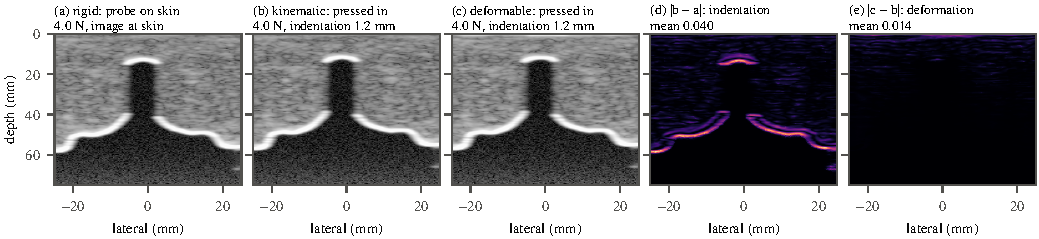
\includegraphics[width=\textwidth]{fig_modes.pdf}
\caption{The three modes at one probe pose (training patient, 4\,N). (a)~Rigid: image at the skin, as in SonoGym.
(b)~Kinematic: probe face pressed 1.2\,mm in, tissue undeformed. (c)~Deformable: pressed in, tissue deformed by the FEM.
(d)~Indentation shifts every echo, including the bone. (e)~Deformation mostly changes the first millimetres under the
probe. Illustration rendered by the simulator, one speckle realisation.}
\label{fig:modes}
\end{figure*}

\subsection{Why not an off-the-shelf soft-body engine?}
\label{sec:engine}
We tested MuJoCo's volumetric soft bodies as the tissue model under a pre-registered gate: same meshes, moduli and
nodal forces as the reference; every case within 10\,\% at 2--5\,N; no inverted elements; one re-solve within the 33\,ms
of a 30\,Hz frame. The default Saint Venant--Kirchhoff material compressed 90--420\,\% too much at 2\,N and inverted
elements in all 24 cases. The stable Neo-Hookean material was within 1.2--4.5\,\% at 2\,N but exceeded 10\,\% in one
5\,N case, inverted elements in 7 of 24 cases, and took 12.5\,s per re-solve, because it time-steps the whole mesh to
rest. Both failed, so the precomputed FEM is kept.

% =====================================================================================================
\section{Preliminary Results}
\label{sec:results}

\subsection{H1: deformation changes a soft-tissue measurement}

\textbf{Set-up.} The structure is the lumbar paraspinal muscle, whose thickness is measured clinically with ultrasound
from the thoracolumbar fascia to the facet joint~\cite{thu2022multifidus}. Per patient we use 6 paraspinal sites and
forces of 1--5\,N (8 and 10\,N are reported only). The image measurement is the distance between the strongest
fascia echo and the bone echo found by an image-only detector, tuned on training patients and frozen. A site is
scored only if the muscle is not cut off by the 75\,mm imaging window and bone is visible at every force; this leaves
2 of the 4 held-out patients measurable (one has no detectable fascia, one no site inside the window). Fig.~\ref{fig:muscle}
shows the measurement on a training patient.

\begin{figure}[t]
\centering
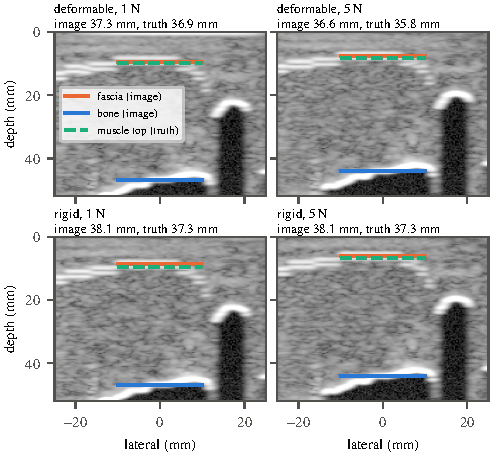
\includegraphics[width=\columnwidth]{fig_muscle.pdf}
\caption{Paraspinal muscle measurement on a training patient at 1 and 5\,N. In \DM\ (top) the image thickness falls
with force, like the truth. In \KM\ (bottom) the probe moves deeper, so every structure moves up, but the thickness
does not change. Illustration, one site.}
\label{fig:muscle}
\end{figure}

\begin{figure}[t]
\centering
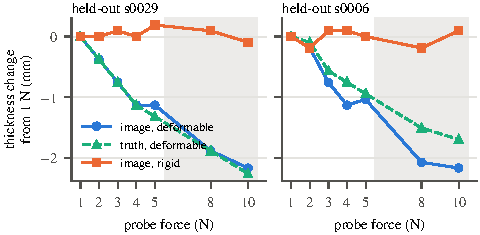
\includegraphics[width=\columnwidth]{fig_thickness.pdf}
\caption{H1 on the held-out patients: thickness change from 1\,N, median over 6 sites. The image follows the true
compression in \DM; the \KM\ (rigid-tissue) image stays flat. Shaded: forces beyond the FEM's validated range.}
\label{fig:thickness}
\end{figure}

\begin{table}[t]
\centering
\caption{H1 on held-out patients (slopes over 1--5\,N, mm/N).}
\label{tab:h1}
\begin{tabular}{@{}lccc@{}}
\toprule
 & s0029 & s0006 & criterion \\
\midrule
detection rate at $\le$2\,N & 1.00 & 1.00 & $\ge 0.5$ \\
median $|\hat t - t|$ at $\le$2\,N (mm) & 0.75 & 2.26 & $<3$ \\
image slope $s_\DM$ & $-0.302$ & $-0.245$ & $<0$ \\
true slope $s_{\rm true}$ & $-0.339$ & $-0.226$ & --- \\
image slope $s_\KM$ & $+0.019$ & $+0.038$ & $|\cdot|\le 0.15$ \\
\bottomrule
\end{tabular}
\end{table}

\textbf{Result.} H1 holds (Table~\ref{tab:h1}, Fig.~\ref{fig:thickness}): the median tracking error
$|s_\DM - s_{\rm true}|$ is 0.075\,mm/N, and the rigid-tissue slopes stay within 0.04\,mm/N of zero. Over 1--5\,N the
effect is about 1.0--1.3\,mm for muscles 38--51\,mm thick. A pre-registered follow-up failed: a single force correction
fitted on training patients does not improve held-out accuracy (median error 1.31 vs 1.32\,mm without the force
term), because constant per-site offsets between image and truth are as large as the force effect.

\subsection{H2: deformation does not change navigation behaviour}

\textbf{Set-up.} Navigation policies are trained in each mode on 2 training patients (300k steps, 2 seeds per mode)
and each is deployed in every mode on the same patients, 64 episodes per policy and mode. Using the training patients
isolates the tissue model from cross-patient generalisation.

\begin{figure}[t]
\centering
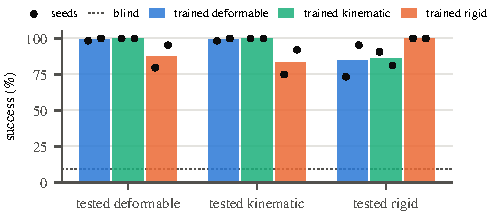
\includegraphics[width=\columnwidth]{fig_nav.pdf}
\caption{Navigation success by training mode (colour) and deployment mode (group). Bars: seed mean; dots: seeds.
\DM- and \KM-trained policies are indistinguishable in every deployment mode.}
\label{fig:nav}
\end{figure}

\begin{table}[t]
\centering
\caption{H2: navigation, policies deployed in \DM\ (64 episodes each).}
\label{tab:h2}
\begin{tabular}{@{}lcccc@{}}
\toprule
trained in & success & final error (mm) & yaw error ($^\circ$) & steps \\
\midrule
\DM\ (seeds 0/1) & 0.98/1.00 & 2.0/1.2 & 2.4/1.7 & 6.3/5.2 \\
\KM\ (seeds 0/1) & 1.00/1.00 & 1.2/1.3 & 1.6/1.6 & 5.5/5.1 \\
\RM\ (seeds 0/1) & 0.80/0.95 & 5.9/1.8 & 5.2/2.5 & 14.9/8.8 \\
\midrule
\multicolumn{5}{@{}l}{deformation-only gap $S(\pi_\DM)-S(\pi_\KM)$: $-1.6$, $0.0$ points (mean $-0.8$)}\\
\multicolumn{5}{@{}l}{gap to rigid training $S(\pi_\DM)-S(\pi_\RM)$: $+18.8$, $+4.7$ points (mean $+11.7$)}\\
\bottomrule
\end{tabular}
\end{table}

\textbf{Result.} H2 is not supported (Table~\ref{tab:h2}, Fig.~\ref{fig:nav}); the gap to rigid training also falls
below the threshold. The decomposition shows where the residual difference comes from: \RM-trained policies lose
about as much when deployed in \KM\ (75.0/92.2\,\% success) as in \DM\ (79.7/95.3\,\%), so their loss is caused by
indentation, not deformation. Two properties of the task limit what it can reveal. First, \DM- and \KM-trained policies
are at the ceiling (98--100\,\%). Second, the controller holds 4\,N and the policy cannot change the force (mean force
3.97--4.00\,N for all policies), so the deformation is a small, nearly constant change near the skin
(Fig.~\ref{fig:modes}e).

\subsection{Other outcomes}
In earlier studies with the same simulator, deformation did not change the reconstruction of a rigid
bone surface with a tracked probe (coverage 88.0 vs 88.8\,\%), and the shift of the bone echo under force was the same
with and without the deformation field in 11 of 12 patients, i.e.\ it was caused by indentation. Navigation policies
reached 100\,\% success on training patients but at most 14.1\,\% on held-out patients.

% =====================================================================================================
\section{Discussion: When Should Deformation Matter?}

All outcomes so far follow one account. Deformation can change an outcome only if (a)~the quantity that the outcome
depends on is itself soft, i.e.\ it moves or changes size under the probe, and (b)~that change is large compared with
the sensing error. Bone fails (a): its echo moves only with the probe, which indentation reproduces. Muscle
thickness satisfies both, with little margin: about 1\,mm of compression against 0.75--2.26\,mm of measurement
error. Navigation at a fixed force fails both, since the target is bony and the policy has no control over how much
the tissue deforms.

This account suggests a practical rule for simulator builders: for bony targets at regulated force, a rigid
simulator that moves the image plane by the indentation is enough; deformation must be simulated when the task
measures or targets soft structures, and especially when the policy chooses the force. It also predicts where policy
behaviour \emph{should} differ, which Stage~2 tests.

% =====================================================================================================
\section{Stage 2 Plan}
\label{sec:plan}

Each item will be pre-registered in the same way before it runs.

\textbf{P1: force-choosing measurement task (tests the account).} The policy places the probe and selects the target
force (1--5\,N), then reports the muscle thickness; reward is the negative error against the \emph{uncompressed}
thickness plus an image-quality term. Prediction: \KM- and \RM-trained policies, which are never penalised for pressing
harder, select higher forces than \DM-trained ones and have a larger negative bias when deployed in \DM. Primary
metric: the same deformation-only gap as H2, applied to measurement error, with the threshold fixed before training.

\textbf{P2: H1 at scale.} Repeat H1 on more TotalSegmentator patients to give a confidence interval for the slope
across anatomies, and report how it varies with fat and muscle thickness.

\textbf{P3: navigation without a ceiling.} Repeat H2 on held-out patients and with more training patients, so that a
deformation-only gap is not hidden by perfect success.

\textbf{P4: sensitivity.} Repeat H1 and P1 with randomised tissue moduli, to test whether conclusions depend on the
shared moduli.

% =====================================================================================================
\section{Limitations}

All results are in simulation; no phantom or patient data anchor the tissue or image model. Moduli are shared across
patients; contact is frictionless and quasi-static; the linear FEM is validated only to about 5\,N; CT is acquired
supine whereas lumbar ultrasound is performed prone; the fascia is a synthetic layer with literature properties.
H1 rests on 2 measurable held-out patients with 6 sites each; H2 on 2 patients, 2 seeds and 300k steps, at the
performance ceiling. One held-out patient was viewed during a visual check of the fascia layer before H1 was run.
Learned policies do not yet generalise across patients, so policy results are for training patients.

\section{Conclusion}
We separated the effect of soft-tissue deformation from that of probe indentation in a patient-specific
robotic-ultrasound simulator. Deformation changes a soft-tissue measurement in a way a rigid simulator cannot
reproduce, but it does not change navigation behaviour at a regulated force. Stage~2 will test whether it changes
behaviour when the policy controls the force.

\bibliographystyle{plainnat}
\bibliography{references}

\end{document}
